\section{Query-dependent GNNs for Multi-hop Reasoning and Retrieval}\label{app:theory}
We provide a detailed explanation about why query-dependent GNNs can be used for multi-hop reasoning and retrieval. Recent studies \citep{huang2023theory,qiuunderstanding} have theoretically proven that query-dependent GNNs are effective for capturing the multi-hop logical associations on KGs to answer queries, such as:
\begin{equation}
    \exists y: \texttt{politician\_of}(\text{Barack Obama},y) \leftarrow \texttt{work\_in}(\text{Barack Obama},z_1) \wedge \texttt{city\_of}(z_1, y),
\end{equation}
where the right part denotes the logical associations can be executed to answer the query on the left, i.e., ``\texttt{politician\_of}(\text{Barack Obama},y)''.

This query is semantic equivalent to the nature language question: ``\texttt{Barack Obama is the politician of which country?}''. By treating the input question as a ``soft query'' (query in nature language), we apply the query-dependent GNN (GFM) to bridge the gap between nature language and logical query. The GFM tries to understand the semantic of the questions and learn to conduct complex logical reasoning (e.g., multi-hop reasoning) on KGs for retrieval~\citep{yasunaga2021qa}. The learned logical associations for reasoning are shown in \Cref{sec:interpretation}.

\input{tables/training_data.tex}
\input{tables/test_data}
\section{Datasets}\label{app:datasets}
\subsection{Multi-hop QA Datasets}\label{app:multi_hop_qa}
Three multi-hop QA datasets are used in our experiments: HotpotQA \citep{yang2018hotpotqa}, MuSiQue \citep{trivedi2022musique}, and 2WikiMultiHopQA (2Wiki) \citep{ho2020constructing}. We provide a brief overview of these datasets below.
\begin{itemize}
    \item HotpotQA \citep{yang2018hotpotqa} is a multi-hop QA dataset that requires reasoning over multiple documents to answer questions. The dataset consists of 97k question-answer pairs, where each question is associated with up to 2 supporting and several distracting documents. The questions are designed to be answerable using multiple pieces of information from the supporting documents.
    \item MuSiQue \citep{trivedi2022musique} is a challenging multi-hop QA dataset with 25k 2-4 hop questions. It requires coherent multi-step reasoning to answer questions that span multiple documents. 
    \item 2WikiMultiHopQA (2Wiki) \citep{ho2020constructing} is a multi-hop QA dataset that requires reasoning over multiple Wikipedia articles to answer questions. The dataset consists of 192k questions, which are designed to be answerable using information from 2 or 4 articles.
\end{itemize}
In experiments, we adhere to the official data split to obtain the training samples and follow existing methods \citep{trivedi2023interleaving,gutiérrez2024hipporag} to use the same 1,000 samples from each validation set to avoid data leakage. We merge the candidate passages as the document corpus for KG-index construction. The statistics of the training and test data are presented in \Cref{tab:training_data} and \Cref{tab:test_data}, respectively.

\subsection{Domain-specific RAG Datasets}\label{app:domain_specific}
To test the generalizability of \ourmethod, we evaluate it on seven domain-specific RAG datasets \citep{friel2024ragbench} including, (1) \emph{biomedical}: PubMedQA \citep{jin-etal-2019-pubmedqa}; (2) \emph{customer support}: DelucionQA \citep{sadat-etal-2023-delucionqa}, TechQA \citep{castelli-etal-2020-techqa}, ExpertQA \citep{malaviya2023expertqa}, EManual \citep{nandy-etal-2021-question-answering}; (3) \emph{general knowledge}: MS Marco \citep{nguyen2016ms}, HAGRID \citep{kamalloo2023hagrid}. We provide a brief overview of these datasets below.

\begin{itemize}
    \item PubMedQA \citep{jin-etal-2019-pubmedqa} is a collection of PubMed research abstracts with corresponding questions paired with 4 abstract chunks.
    \item  DelucionQA \citep{sadat-etal-2023-delucionqa} is a domain-specific RAG dataset leveraging Jeep’s 2023 Gladiator model manual as the source of knowledge, where each question is associated with 4 context documents and only 1 relevant passage.
    \item TechQA \citep{castelli-etal-2020-techqa} is a collection of real-world user questions posted on IBMDeveloper and DeveloperWorks forums, along with 10 technical support documents relating to each question.
    \item ExpertQA \citep{malaviya2023expertqa} is a collection of curated questions from domain experts in various fields of science, arts, and law. The dataset also contains expert-curated passages relevant to each question.
    \item EManual \citep{nandy-etal-2021-question-answering} is a question-answering dataset comprising consumer electronic device manuals and realistic questions about them composed by human annotators, where each question is related with up to 3 context documents.
     \item MS Marco \citep{nguyen2016ms} is an open-domain question-answering dataset sourced from Bing search engine user query logs. Each question is associated with 10 context passages retrieved via Bing web search.
    \item HAGRID \citep{kamalloo2023hagrid} is a multi-lingual information retrieval dataset with questions and passages from MIRACL \citep{zhang2022making}.
\end{itemize}
In experiments, we use test sets constructed by RAGBench \citep{friel2024ragbench} and merge all the candidate passages as document corpus for KG-index construction. The statistics of the test dataset are detailed in \Cref{tab:test_data}.

\section{Baselines}\label{app:baselines}
In experiments, we compare with several widely used retrieval methods under three categories: (1) \emph{single-step naive methods}: BM25 \citep{robertson1994some}, Contriever \citep{izacardunsupervised}, GTR \citep{ni2022large}, ColBERTv2 \citep{santhanam2022colbertv2}, RAPTOR \citep{sarthiraptor}, Proposition \citep{chen-etal-2024-dense}; (2) \emph{graph-enhanced methods}: GraphRAG (MS) \citep{edge2024local}, LightRAG \citep{guo2024lightrag}, HippoRAG \citep{gutiérrez2024hipporag}; (3) \emph{multi-step methods}: Adaptive-RAG \citep{jeong2024adaptive}, FLARE \citep{jiang2023active}, and IRCoT \citep{trivedi2023interleaving}. The detailed introduction of the baselines is as follows.

\noindent\textbf{Single-step Naive Methods} are widely adopted in real-world applications due to their great efficiency and generalizability. 
\begin{itemize}
    \item BM25 \citep{robertson1994some} is a classic information retrieval method based on the probabilistic model that ranks a set of documents based on the query terms frequency appearing in each document.
    \item Contriever \citep{izacardunsupervised} trains a dense retriever with contrastive learning on a large-scale corpus to retrieve relevant documents for a given query.
    \item GTR \citep{ni2022large} develops a scale-up T5-based dense retriever that could generalize across different datasets and domains.
    \item ColBERTv2 \citep{santhanam2022colbertv2} is a state-of-the-art dense retriever that couples an aggressive residual compression mechanism with a denoised supervision strategy to simultaneously improve the retrieval quality.
    \item RAPTOR \citep{sarthiraptor} is an LLM-augmented retriever that recursively embeds, clusters, and summarizes chunks of text, constructing a tree with differing levels of summarization to enable accurate retrieval.
    \item Proposition \citep{chen-etal-2024-dense} enhances the performance of dense retrievers by leveraging LLMs to generate a natural language proposition that captures the essential information of the document.
\end{itemize}

\noindent\textbf{Graph-enhanced Methods} design a retriever that is built upon a graph structure to conduct effective retrieval and reasoning.
\begin{itemize}
    \item GraphRAG (MS) \citep{edge2024local} is a graph-enhanced retrieval method originally proposed by Microsoft. It builds a graph structure from the document corpus and use hierarchical community detection to cluster the documents into communities and generate a summary for each community. The summary together with the original documents are retrieved by the retriever for LLM generation. 
    \item LightRAG \citep{guo2024lightrag} is an innovative graph-enhanced RAG method that incorporates graph structures into text indexing and retrieval, enabling efficient retrieval of entities and their relationships. It employs a dual-level retrieval system to gather both low-level and high-level knowledge for LLM generation.
    \item HippoRAG \citep{gutiérrez2024hipporag} is a state-of-the-art, training-free graph-enhanced retriever that uses the Personalized PageRank algorithm to assess entity relevance to a query and performs multi-hop retrieval on a document-based knowledge graph. It can be directly applied to various datasets.
\end{itemize}

\noindent\textbf{Multi-step Methods} are designed to conduct multi-hop reasoning by iteratively retrieving and reasoning over documents, which can be integrated with arbitrary retrieval methods.
\begin{itemize}
    \item Adaptive-RAG \citep{jeong2024adaptive} proposes an adaptive multi-step retrieval method that can dynamically select the most suitable retrieval strategy based on the complexity of the query.
    \item FLARE \citep{jiang2023active} introduces a multi-step retrieval method that actively decide when and how to retrieve documents. It also predicts the future content to the guide the retrieval in next steps. 
    \item IRCoT \citep{trivedi2023interleaving} is a powerful multi-step retrieval pipeline that integrates the retrieval with the chain-of-thought (CoT) reasoning of LLMs. It guides the retrieval with CoT and in turn using retrieved documents to improve CoT. IRCoT can be compatible with arbitrary retrievers to conduct multi-step retrieval and reasoning.
\end{itemize}

\section{Implementations and Training Details}\label{app:implementation}

\subsection{Training Data Construction}\label{app:kg_index}
We extract 60,000 samples from the training set of HotpotQA, MuSiQu, and 2Wiki to construct KG-indexes and conduct large-scale training. Specifically, we merge the candidate passages as the document corpus. In the KG-index construction, we use the GPT-4o-mini \citep{gpt4o} with the OpenIE prompts described in HippoRAG \citep{gutiérrez2024hipporag} to extract the entities, relations, and triples from the document corpus. Then, we use the ColBERTv2 \citep{santhanam2022colbertv2} to conduct the entity resolution by computing the similarity between entities as
\begin{equation}
    s(e_i, e_j) = \text{Emb.}(e_i)^{\top} \text{Emb.}(e_j), 
\end{equation}
where a new triple $(e_i, \texttt{equivalent}, e_j)$ is generated if $s(e_i, e_j) > \tau$ and $e_i \neq e_j$. We set the threshold $\tau$ as 0.8 in our experiments. We divide the samples into groups of approximately 1k questions and 10k documents each to control the constructed KG-index size. In the end, we obtain 60 different KG-indexes and associated question-document pairs for model training.

\subsection{Model Settings}\label{app:model_settings}
In \ourmethod, the GFM is implemented as a 6-layer query-dependent GNN with the hidden dimension of 512, DistMult message function, and sum aggregation. The relation update function $g^{l}(\cdot)$ is implemented as a 2-layer MLP. We use the all-mpnet-v2 as the sentence embedding model with a dimension of 768. The total training parameters of the GFM is 8M. In the retrieval stage, we select top $T=20$ entities for the document ranker.

\input{tables/settings}

\subsection{Training Settings}\label{app:training_settings}
In KG completion pre-training, we randomly sample triples $(e, r, t)$ from knowledge graphs and mask out either the head or the tail entity to create a synthetic query $q = (e, r, ?)$ and answer $a = \{e\}$ in a self-supervised manner. For example, given a triple (\texttt{Barack Obama}, \texttt{born\_in}, \texttt{Honolulu}), we can create a query as $(\texttt{Barack Obama}, \texttt{born\_in}, ?)$, which is encoded as a sentence embedding and fed into the GFM to predict the target entity \texttt{Honolulu} on graphs.

In supervised document retrieval fine-tuning, we obtain natural language questions and supporting documents from the multi-hop QA datasets. For each question, we identify the entities from its supporting documents as the targets. For instance, given the question \textit{``Where was Barack Obama born in?''}, we can extract two entities such as \texttt{[Honolulu, USA]} from its supporting documents (e.g., Doc.~2 in \Cref{fig:framework}). The GFM is trained to maximize the likelihood of these two target entities.

In the self-supervised KG completion pre-training, the GFM is trained on the mixture of 60 constructed KG-indexes for 30,000 steps. Then, we conduct the supervised document retrieval fine-tuning on the labeled question-document pairs for 5 epochs. The weight $\alpha$ between losses is set to 0.3. We use AdamW optimizer, learning rate of 5e-4 with batch sizes of both training stages set to 4. Each batch contains only one KG-index and training samples associated to it, where we randomly sample from different KG-indexes during training. The model is trained on 8 NVIDIA A100s (80G) with 14 hours pre-training and 5 hours supervised fine-tuning. The detailed settings are summarized in \Cref{tab:settings}.



\section{Additional Experiments}\label{app:additional_experiments}

\begin{table}[]
    \centering
    \caption{Comparison of different sentence embedding models used in \ourmethod.}
    \label{tab:text-emb}
    % \resizebox{\columnwidth}{!}{%
    \begin{tabular}{@{}l|cc|cc|cc@{}}
    \toprule
    \multirow{2}{*}{Sentence Embedding Model} & \multicolumn{2}{c|}{HotpotQA} & \multicolumn{2}{c|}{MuSique}  & \multicolumn{2}{c}{2Wiki}     \\ \cmidrule(l){2-7} 
                                              & R@2           & R@5           & R@2           & R@5           & R@2           & R@5           \\ \midrule
    sentence-transformers/all-mpnet-base-v2   & \textbf{70.2} & \textbf{82.1} & 46.0 & 55.1 & \textbf{81.1} & 85.6 \\
    BAAI/bge-large-en                         & 68.1          & 81.1          & 45.9          &  \textbf{55.9}          & 80.7          & \textbf{86.3}          \\
    Alibaba-NLP/gte-Qwen2-1.5B-instruct       & 69.9          & 81.5          & 46.0          & 55.0          & 79.8          & 86.2          \\
    Alibaba-NLP/gte-Qwen2-7B-instruct         & 68.5          & 81.5          & 45.5          & 55.1          & 80.8          & 85.6          \\
    nvidia/NV-Embed-v2                        & 69.2          & 81.4          & \textbf{46.3}          & 54.9          & 80.3          & 85.5          \\ \bottomrule
    \end{tabular}%
    % }
    \end{table}


    \begin{table}[]
        \centering
        \caption{Comparison of \ourmethod with pre-trained and fine-tuned sentence embedding models.}
        \label{tab:text_emb_ablation}
        % \resizebox{\columnwidth}{!}{%
        \begin{tabular}{@{}l|cc|cc|cc@{}}
        \toprule
        \multirow{2}{*}{Method}    & \multicolumn{2}{c|}{HotpotQA} & \multicolumn{2}{c|}{MuSiQue}  & \multicolumn{2}{c}{2Wiki}     \\ \cmidrule(l){2-7} 
                                   & R@2           & R@5           & R@2           & R@5           & R@2           & R@5           \\ \midrule
        \ourmethod                    & \textbf{78.3} & \textbf{87.1} & \textbf{49.1} & \textbf{58.2} & \textbf{90.8} & \textbf{95.6} \\ \midrule
        all-mpnet-v2 (pre-trained) & 59.4          & 73.3          & 33.2          & 46.3          & 48.5          & 59.4          \\
        all-mpnet-v2 (finetuned)   & 67.0          & 82.3          & 41.7          & 55.0          & 65.1          & 76.7          \\ \bottomrule
        \end{tabular}%
        % }
        \end{table}
\subsection{Effectiveness of Different Sentence Embeddings}\label{app:text_embeddings}

In this section, we first study the effectiveness of different sentence embeddings in the GFM. We compare the all-mpnet-v2 \citep{all-mpnet-v2}, bge-large-en \citep{bge_embedding}, gte-Qwen2-1.5B-instruct and gte-Qwen2-7B-instruct \citep{li2023towards} as well as NV-Embed-v2 \citep{lee2024nv}. We download the official pre-trained model from the Huggingface\footnote{\url{https://huggingface.co/}}. The details of the models are shown in \Cref{tab:text-emb}. From the results, we can  observe that the performance variance between different sentence embeddings is relatively small, where the all-mpnet-v2 achieves the best performance with respect to 3 metrics. This indicates that \ourmethod is not sensitive to the choice of sentence embedding models. In experiments, we use the all-mpnet-v2 as the default sentence embedding model due to its efficiency. However, it has relative smaller context-size (512) which limits the length of input text. We leave the exploration of larger context-size sentence embedding models (e.g., NV-Embed-v2 with 32k context) for future work.

Then, we expand our ablation study to compare \ourmethod with variants without GNN and using solely the pre-trained all-mpnet-v2 embeddings and those fine-tuned on multi-hop QA data, respectively. The results are shown in \Cref{tab:text_emb_ablation}. We can observe that GNN plays a crucial role in retrieval. The sentence embedding model all-mpnet-v2 is pre-trained on large-scale text data and could potentially see the QA data. However, it is not specifically trained for the multi-hop QA task, which leads to suboptimal performance in capturing the relationship between question and supporting documents. The fine-tuned all-mpnet-v2 achieves better performance than the pre-trained one by supervised fine-tuning on the multi-hop QA data, but still inferior to \ourmethod. This indicates that the GNN can effectively capture the relationship between knowledge and conduct multi-hop reasoning, which is not achievable by simply using the sentence embedding model.

\subsection{Effectiveness of Different Training Strategies}\label{app:pre-training}
In this section, we first study the effectiveness of the two training tasks used in \ourmethod. We compare the performance by only conducting the KG completion pre-training (\ourmethod $w/o$ Fine-tune) and supervised document retrieval fine-tuning (\ourmethod $w/o$ Pre-train). The results are shown in \Cref{tab:pre-train}. The results show that removing the supervised document retrieval fine-tuning significantly decreases the performance of \ourmethod. This highlights the importance of supervised fine-tuning, as it enables the model to understand users' queries and better capture the relevance between questions and knowledge for improved retrieval. 

\begin{table}[]
    \centering
    \caption{Effectiveness of KGC pre-training and supervised retrieval fine-tuning in \ourmethod.}
    \label{tab:pre-train}
    % \resizebox{\columnwidth}{!}{%
    \begin{tabular}{@{}l|cc|cc|cc@{}}
    \toprule
    \multirow{2}{*}{Method} & \multicolumn{2}{c|}{HotpotQA} & \multicolumn{2}{c|}{MuSique}  & \multicolumn{2}{c}{2Wiki}     \\ \cmidrule(l){2-7} 
                                              & R@2           & R@5           & R@2           & R@5           & R@2           & R@5           \\ \midrule
    \ourmethod                                & \textbf{78.3} & \textbf{87.1} & \textbf{49.1} & 58.2          & \textbf{89.1} & \textbf{92.8} \\ 
    \ourmethod $w/o$ Retrieval Fine-tune                &   21.0            &  32.8             &     18.3          &   25.9            &  44.6             &   53.4            \\
    \ourmethod $w/o$ KGC Pre-train                & 77.8          & 86.5          & 48.3          & \textbf{58.3} & 88.3          & 92.5          \\\bottomrule
    \end{tabular}%
    % }
    \end{table}

    \begin{table}[]
        \centering
        \caption{Knowledge graph completion result of different training strategies.}
        \label{tab:kgc}
        % \resizebox{\columnwidth}{!}{%
        \begin{tabular}{@{}l|cccc@{}}
        \toprule
        Method                                                              & MRR            & Hits@1         & Hits@3         & Hits@10        \\ \midrule
        \ourmethod                                                            & 0.193          & 0.138          & 0.221          & 0.293          \\
        \ourmethod $w/o$ Retrieval Fine-tune                                            & \textbf{0.304} & \textbf{0.234} & \textbf{0.323} & \textbf{0.451} \\
        \begin{tabular}[c]{@{}l@{}}\ourmethod $w/o$ KGC Pre-train\end{tabular} & 0.029          & 0.007          & 0.022         & 0.067           \\ \bottomrule
        \end{tabular}%
        % }
        \end{table}

Although the pre-training has a relatively small impact on the final performance, its primary purpose is to learn the general graph reasoning ability, following previous studies like ULTRA \cite{galkintowards}. This would enhance the generalization and robustness of the GFM, which could be beneficial to its performance on other tasks, such as knowledge graph completion. To further validate this, we conduct an ablation study to compare \ourmethod with different training strategies on the knowledge graph completion task. We report the knowledge graph completion (KGC) performance on the KG-index from the test set of the HotpotQA dataset. The results are shown in \Cref{tab:kgc}. 

From the knowledge graph completion results, we can observe that the \ourmethod undergoes only the pre-training (\ourmethod $w/o$ Fine-tune) achieves the best performance, which indicates that the pre-training is effective in learning the general graph reasoning ability. The performance of \ourmethod with only supervised fine-tuning (\ourmethod $w/o$ Pre-train) is significantly lower than that of \ourmethod with pre-training. This indicates that the supervised fine-tuning is only learning the specific downstream task, which would limit the generalization ability of \ourmethod as the foundation model. The GFM trained with both pre-training and supervised fine-tuning achieves the second-best performance on the knowledge graph completion task and the best performance on the multi-hop QA task. This indicates that both training strategies are essential for \ourmethod to learn the general graph reasoning ability and benefit specific downstream tasks.


\subsection{Effectiveness of Loss Weights}\label{app:loss_weight}
In this section, we examine the effectiveness of the weights assigned to the BCE loss and ranking loss in training \ourmethod. We compare performance by varying the weight $\alpha$ between the two losses: $\gL=\alpha\gL_{\text{BCE}} + (1-\alpha)\gL_{\text{RANK}}$, with results presented in \Cref{tab:loss_weight}. The findings indicate that using only either the BCE loss or ranking loss leads to suboptimal performance ($\alpha=0~\text{or}~1$). The best performance occurs when $\alpha$ is set to 0.3, which aligns with previous studies \citep{lin2024understanding} suggesting that a smaller weight for BCE loss is preferable when positive samples are rare in the training data.

\input{tables/loss_weight.tex}

\subsection{Effectiveness of Ranking Methods}\label{app:ranking_method}
In this section, we investigate the effectiveness of different ranking methods based on inverted index used in \ourmethod. We compare four ranking methods including (1) \emph{IDF + Top-T Pred}: Our proposed method (\cref{eq:top-T,eq:entity_weight,eq:doc_score}), which maps the top-T entities predicted by GFM to documents using inverse document frequency (IDF)-weighted scores. (2) \emph{IDF + All Pred}: Uses all predicted entities from GFM and weights them by IDF ($w/o$ \cref{eq:top-T}). (3) \emph{Top-T Pred}: Uses only the top-T predicted entities without applying IDF weighting ($w/o$ \cref{eq:entity_weight}). (4) \emph{All Pred}: Use all entity predictions and directly map to document scores ($w/o$ \cref{eq:top-T,eq:entity_weight}). The results are shown in \Cref{tab:ranking}. The results show that the proposed \emph{IDF + Top-k Pred} performs the best. This indicates that the inverted index is a crucial component of \ourmethod, which serves as a bridge between structured reasoning over KGs and the unstructured documents required by LLMs, necessitating a careful design.

We acknowledge the potential alternatives, and as a promising future direction, we plan to explore end-to-end models that can jointly reason over structured and unstructured knowledge without relying on an explicit inverted index.

\begin{table}[h]
\centering
\caption{Comparison of different ranking methods.}
\label{tab:ranking}
% \resizebox{\columnwidth}{!}{%
\begin{tabular}{@{}lcccccc@{}}
\toprule
\multirow{2}{*}{Ranking Method} & \multicolumn{2}{c}{HotpotQA} & \multicolumn{2}{c}{MuSiQue} & \multicolumn{2}{c}{2Wiki} \\ \cmidrule(l){2-7} 
                                & R@2           & R@5          & R@2          & R@5          & R@2         & R@5         \\ \midrule
IDF + Top-T Pred (\ourmethod)     & \textbf{78.3} & \textbf{87.1} & \textbf{49.1} & \textbf{58.2} & \textbf{90.8} & \textbf{95.6} \\ \midrule
IDF + All Pred ($w/o$ \cref{eq:top-T})                 & 68.1          & 71.4         & 35.8         & 41.2         & 86.0        & 87.5        \\
Top-T Pred ($w/o$ \cref{eq:entity_weight})                     & 71.6          & 78.6         & 46.3         & 52.5         & 74.7        & 78.1        \\
All Pred ($w/o$ \cref{eq:top-T,eq:entity_weight})                      & 77.6          & 82.9         & 41.1         & 46.9         & 88.6        & 90.4        \\ \bottomrule
\end{tabular}%
% }
\end{table}

\subsection{Ablation Study of Training Datasets}\label{app:training_data_ablation}
We further conducted ablation studies where \ourmethod is trained separately on each dataset, and we report performance across all three benchmarks. Results are shown \Cref{tab:dataset_ablation}. These results show that \ourmethod not only performs well on the trained datasets, but also generalizes well to other datasets.  More importantly, the model trained on multi-domain datasets performs competitively across all datasets, validating its ability to generalize effectively across domains and benefit from training on diverse KGs by learning generalizable reasoning ability across domains.

\begin{table}[]
\centering
\caption{Ablation study of \ourmethod trained on each dataset. Best results are highlighted in \textbf{bold}. The second best is \underline{underlined}.}
\label{tab:dataset_ablation}
% \resizebox{\columnwidth}{!}{%
\begin{tabular}{@{}c|cc|cc|cc@{}}
\toprule
Test Dataset     & \multicolumn{2}{c|}{HotpotQA} & \multicolumn{2}{c|}{MuSiQue}  & \multicolumn{2}{c}{2Wiki}     \\ \midrule
Training Dataset & R@2           & R@5           & R@2           & R@5           & R@2           & R@5           \\ \midrule
HotpotQA         & \textbf{79.3} & \textbf{87.8} & 46.9          & 57.2          & 86.6          & 92.4          \\
MusiQue          & 68.8          & 81.8          & {\ul 47.6}    & {\ul 57.5}    & 84.4          & 89.6          \\
2Wiki            & 72.2          & 77.9          & 46.6          & 55.5          & {\ul 89.3}    & {\ul 93.2}    \\ \midrule
All              & {\ul 78.3}    & {\ul 87.1}    & \textbf{49.1} & \textbf{58.2} & \textbf{90.8} & \textbf{95.6} \\ \bottomrule
\end{tabular}%
% }
\end{table}

\subsection{Model Transferability}\label{app:trans}
\input{tables/transferability}
In this section, we evaluate \ourmethod's transferability by conducting domain-specific fine-tuning on the training split of dataset on each domain. As shown in \ref{tab:trans}, \ourmethod performs well in zero-shot generalization, with further improvements achieved through domain-specific fine-tuning. This highlights its transferability when adapted to domain-specific datasets.

\input{tables/model_size.tex}
\subsection{Details of Model Neural Scaling}\label{app:scaling}
In this section, we provide more details on the neural scaling experiments. We evaluate the changes of the model performance with respect to different parameter sizes and training data sizes. In \ourmethod, the model parameter sizes are primarily influenced by the hidden dimension of the GFM. Thus, we vary the dimension from 32 to 512 which results in the model parameter sizes ranging from 0.08M to 8M. The detailed settings are shown in \Cref{tab:model_size}. We test models with different sizes on different scales of training data ranging from 3k to 45k samples. We separately report the fitted trend line of performance changing with model parameter size and training data size in \Cref{fig:scaling_separate}. From the trend line, we can observe that the performance of \ourmethod increases with the model parameter size and training data size. Meanwhile, with the larger model parameter size a larger training data size is required to achieve the best performance. This indicates that the performance of \ourmethod can be further improved by scaling up the model size and training data simultaneously.

To further investigate architectural design, we varied the number of GNN layers from 1 to 8 while keeping the hidden dimension fixed (512), and evaluated model performance across all datasets. The results are shown in \Cref{tab:layers}. We observe that performance generally improves with deeper GNN layers, which we attribute to both the increased model sizes and the ability to capture more complex multi-hop associations. This trend aligns with the neural scaling laws observed in foundation models, where larger parameter counts typically yield better generalization.

Interestingly, we find that performance peaks around 4 layers in some cases. As discussed in \Cref{app:theory} and \Cref{sec:interpretation}, \ourmethod is designed to capture logical associations from KGs through multi-hop message passing. However, since the maximum number of reasoning hops required by our datasets is 4, additional layers beyond this offer limited benefit, likely due to the absence of higher-hop training signals. This finding supports our hypothesis that \ourmethod effectively learns query-relevant multi-hop reasoning paths, and that deeper architectures may not improve performance without datasets requiring more complex reasoning.
In summary, these results demonstrate the effectiveness and interpretability of the proposed GNN-based architecture, and confirm that both model capacity and logical expressibility contribute to \ourmethod’s strong performance. We recognize the potential of other architectural designs and aim to explore them in the future, inspiring the community to do the same.


\begin{figure*}[]
    \centering
    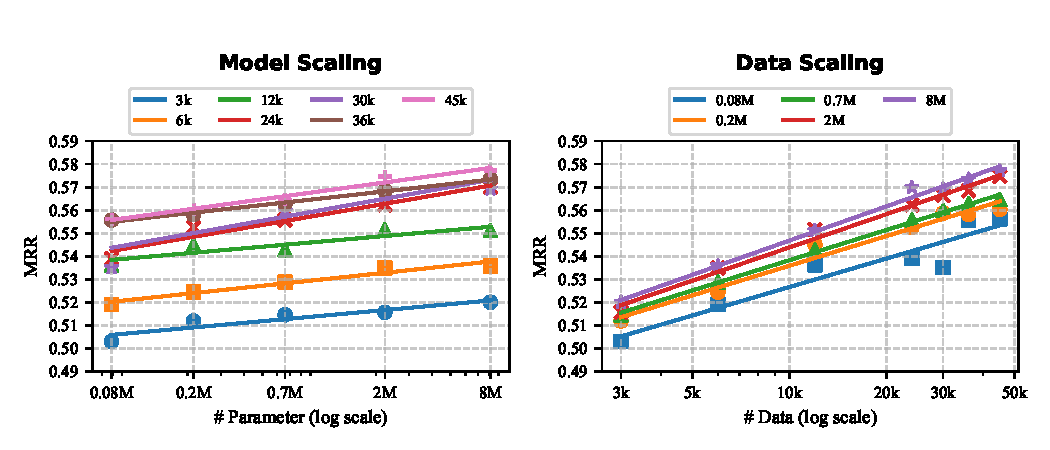
\includegraphics[width=5.5in]{images/scaling_separate.pdf}
    % \vspace{-.6cm}
    \caption{The illustration of the model and data scaling law of \ourmethod.}
    \label{fig:scaling_separate}
    % \vspace{-0.5cm}
\end{figure*}


    \begin{table}[]
\centering
\caption{The different number of layers with corresponding model size and performance for scaling law analysis.}
\label{tab:layers}
% \resizebox{\columnwidth}{!}{%
\begin{tabular}{@{}c|cc|cc|cc|cc@{}}
    \toprule
Hidden Dim. = 512     & \multicolumn{2}{c|}{Averge}   & \multicolumn{2}{c|}{HotpotQA} & \multicolumn{2}{c|}{MuSiQue}  & \multicolumn{2}{c}{2Wiki}     \\ \midrule
L-Layer       & R@2           & R@5           & R@2           & R@5           & R@2           & R@5           & R@2           & R@5           \\ \midrule
1-layer (3M)  & 53.9          & 66.7          & 59.3          & 74.2          & 40.7          & 50.2          & 61.8          & 75.7          \\
2-layer (4M)  & 69.9          & 78.6          & 73.6          & 85.4          & 47.6          & 57.0          & 88.6          & 93.3          \\
4-layer (6M)  & 72.2          & \textbf{80.1} & 78.4          & 87.8          & 49.3          & \textbf{60.1} & 88.8          & 92.5          \\
6-layer (8M)  & 71.9          & 79.6          & 78.0          & 87.0          & 48.4          & 58.7          & 89.3          & 93.1          \\
8-layer (10M) & \textbf{73.0} & 79.9          & \textbf{79.7} & \textbf{87.8} & \textbf{49.7} & 59.1          & \textbf{89.5} & \textbf{92.8}\\ \bottomrule
\end{tabular}%
% }
\end{table}

\begin{figure*}[t]
    \centering
    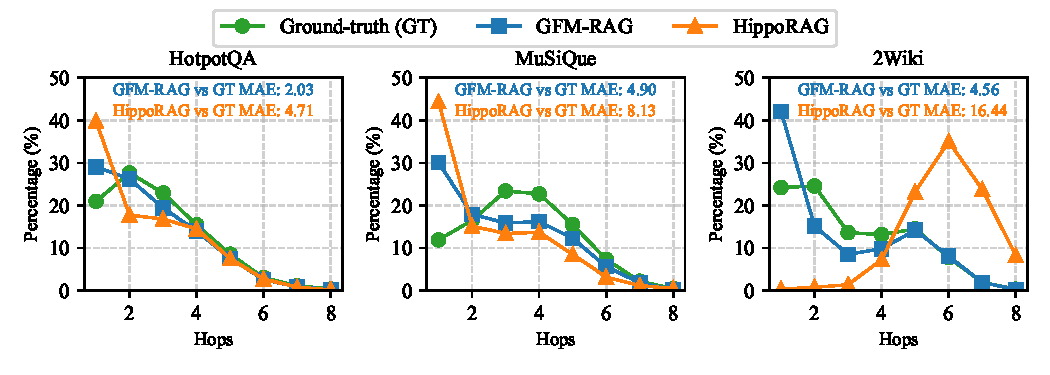
\includegraphics[width=5.5in]{images/prediction_hops_analysis.pdf}
    % \vspace{-.6cm}
    \caption{Statistics of the prediction hops of \ourmethod and HippoRAG against the ground-truth.}
    \label{fig:vis_hops}
    % \vspace{-0.5cm}
\end{figure*}
\subsection{Visualization of the Distribution of Multi-hop Prediction}\label{app:multi_hop}
In this section, we visualize the distribution of the number of hops in the multi-hop reasoning process of \ourmethod. We calculate the number of hops in the ground-truth reasoning path required for each question in the test set of HotpotQA, MuSiQue, and 2Wiki. Then, we compare the distribution of the number of hops in the reasoning path of the ground-truth and the predicted reasoning path by \ourmethod as well as HippoRAG.
%
The results are shown in \Cref{fig:vis_hops}. We can observe that the distribution of \ourmethod is closely aligned to the ground-truth, which indicates that \ourmethod can effectively conduct the multi-hop reasoning within a single step. Meanwhile, the distribution of HippoRAG is relatively different from the ground-truth, especially in 2Wiki dataset. This indicates that HippoRAG may not be able to effectively capture the complex relationship to conduct multi-hop reasoning on graphs.

\begin{table}[]
\centering
\caption{The cost of the KG-index construction.}
\label{tab:kg_index_cost}
% \resizebox{\columnwidth}{!}{%
\begin{tabular}{@{}ccc@{}}
\toprule
LLM         & Price per 10k docs. & Total Price \\ \midrule
GPT-4o-mini & \$2.93                 & \$216        \\ \bottomrule
\end{tabular}%
% }
\end{table}

\begin{table}[]
\centering
\caption{Token cost comparison for index construction}
\label{tab:token_cost}
% \resizebox{\columnwidth}{!}{%
\begin{tabular}{@{}cc@{}}
\toprule
Method     & \# Tokens per 10k documents \\
\midrule
LightRAG   & 55M                        \\
GraphRAG   & 76M                        \\
\ourmethod & \textbf{48M}              \\ \bottomrule
\end{tabular}%
% }
\end{table}

\begin{table}[]
\centering
\caption{Graph Indexing time comparison.}
\label{tab:index_time}
% \resizebox{\columnwidth}{!}{%
\begin{tabular}{@{}cc@{}}
\toprule
Method        & Indexing time (s) \\ \midrule
LightRAG      & 1430.32           \\
GraphRAG (MS) & 1796.43           \\
\ourmethod       & \textbf{93.55}    \\ \bottomrule
\end{tabular}%
% }
\end{table}

\begin{table}[]
\centering
\caption{Comparison of the model performance under the KG-index constructed by different LLMs. }
\label{tab:kg_index_llm}
% \resizebox{\columnwidth}{!}{%
\begin{tabular}{@{}l|cc|cc|cc@{}}
\toprule
\multirow{2}{*}{Method}  & \multicolumn{2}{c|}{HotpotQA} & \multicolumn{2}{c|}{MuSiQue} & \multicolumn{2}{c}{2Wiki} \\ \cmidrule(l){2-7} 
                         & R@2           & R@5           & R@2           & R@5          & R@2         & R@5         \\ \midrule
GFM-RAG (gpt-4o-mini)    & 78.3          & 87.1          & 49.1          & 58.2         & 90.8        & 95.6        \\
HippoRAG (gpt-4o-mini)   & 62.2          & 79.3          & 41.7          & 53.6         & 72.1        & 89.5        \\ \midrule
GFM-RAG (gpt-3.5-trubo)  & 75.6          & 84.7          & 46.1          & 55.8         & 85.2        & 90.4        \\
HippoRAG (gpt-3.5-trubo) & 60.5          & 77.7          & 40.9          & 51.9         & 70.7        & 89.1        \\ \bottomrule
\end{tabular}%
% }
\end{table}
\subsection{Cost and Impact of LLMs on KG-index Construction}\label{app:cost}

In this section, we first analyze the cost of the KG-index construction. In experiments, we utilize GPT-4o-mini\footnote{\url{https://platform.openai.com/docs/models/o4-mini}} for OpenIE extraction and construct the KG-index for 737,310 documents. The cost is shown in \Cref{tab:kg_index_cost,tab:token_cost}. Specifically, we find that constructing the KG-index requires approximately 48M tokens per 10k documents, which costs around \$2.6 using GPT-4o-mini. LightRAG and GraphRAG cost 57M tokens and 76M tokens, respectively. Compared to other methods, \ourmethod is more cost-effective as it does not require generating community-level summaries. In addition, we compare the graph index construction time of \ourmethod in \Cref{tab:index_time}. Results show that \ourmethod benefits from the quick index process during retrieval, as it does not construct a traditional vector database to store documents and entities.

Admittedly, using an LLM for KG index construction incurs computational costs. However, KG construction has been extensively studied, and numerous alternative methods exist that do not rely on LLMs \citep{zhong2023comprehensive}. Our implementation offers an easy interface for integration with any KG construction tools. We would explore the use of other KG construction methods in future work.

We further analyze the impact of LLMs used for KG-index construction on the performance of \ourmethod. We conduct experiments using different LLMs for KG-index construction, including GPT-4o-mini and GPT-3.5-turbo\footnote{\url{https://platform.openai.com/docs/models/gpt-3-5-turbo}}. Then, we reevaluate the performance of \ourmethod and HippoRAG with the constructed KG-index. The results are shown in \Cref{tab:kg_index_llm}. From the results, the performance of both methods on the KG extracted by GPT-4o-mini is higher than the ones by GPT-3.5-turbo. This supports the opinion that GPT-4o-mini generally outperforms GPT-3.5-turbo in constructing high quality KG-index, which is crucial for the graph-enhanced retrieval. However, the performance of \ourmethod is significantly higher than HippoRAG under both KG-indexes. This indicates that \ourmethod is more robust to the quality of the KG-index, demonstrating the effectiveness of the GFM in graph reasoning and retrieval. 

\section{Prompts}\label{app:prompt}

In experiments, we follow the prompts used in HippoRAG \citep{gutiérrez2024hipporag} to extract the triples from the document corpus, which is shown in \Cref{tab:prompt}.

\begin{table}
    \centering
    \begin{tcolorbox}[title=OpenIE Prompt]
    \small
    \begin{lstlisting}
## Instruction:  
Your task is to construct an RDF (Resource Description Framework) graph from the given passages and named entity lists. Respond with a JSON list of triples, with each triple representing a relationship in the RDF graph. Pay attention to the following requirements: 
- Each triple should contain at least one, but preferably two, of the named entities in the list for each passage.
- Clearly resolve pronouns to their specific names to maintain clarity.  

Convert the paragraph into a JSON dict, it has a named entity list and a triple list.

## One-Shot Demonstration:
Paragraph:
```
Radio City
Radio City is India's first private FM radio station and was started on 3 July 2001. It plays Hindi, English and regional songs. Radio City recently forayed into New Media in May 2008 with the launch of a music portal - PlanetRadiocity.com that offers music related news, videos, songs, and other music-related features.
```
{
    "named_entities":
    ["Radio City", "India", "3 July 2001", "Hindi", "English", "May 2008", "PlanetRadiocity.com"]
}
{
    "triples": [
            ["Radio City", "located in", "India"],
            ["Radio City", "is", "private FM radio station"],
            ["Radio City", "started on", "3 July 2001"],
            ["Radio City", "plays songs in", "Hindi"],
            ["Radio City", "plays songs in", "English"]
            ["Radio City", "forayed into", "New Media"],
            ["Radio City", "launched", "PlanetRadiocity.com"],
            ["PlanetRadiocity.com", "launched in", "May 2008"],
            ["PlanetRadiocity.com", "is", "music portal"],
            ["PlanetRadiocity.com", "offers", "news"],
            ["PlanetRadiocity.com", "offers", "videos"],
            ["PlanetRadiocity.com", "offers", "songs"]
    ]
}

## Input
Convert the paragraph into a JSON dict, it has a named entity list and a triple list. Paragraph:
```
INPUT PASSAGE
```
        \end{lstlisting}
    \end{tcolorbox}
    \caption{The prompt for OpenIE extraction.}
\label{tab:prompt}
\end{table}

\section{Limitations}\label{app:Limitation}

The limitations of \ourmethod are as follows: (1) The construction of KG-index can be costly and time-consuming, especially when using LLMs for OpenIE extraction. We would explore the use of efficient KG construction methods in future work and optimize the construction process. (2) The model size of the \ourmethod is relatively small (8M) compared to other foundation models like large language models with billions of parameters. Although it is not faired to directly compare the GNN-based model with transformer-based LLMs, we would explore the scaling of \ourmethod in future work to improve its performance and generalizability. (3) \ourmethod is only evaluated on multi-hop QA tasks and KG completion tasks. We would explore the capabilities of \ourmethod in other tasks such as knowledge graph question answering and knowledge graph reasoning in future work to validate its effectiveness as a foundation model.

\input{sections/statement.tex}